\documentclass{article}

\usepackage[letterpaper,left=1.5cm,right=1.5cm]{geometry}
\usepackage[utf8]{inputenc}
\usepackage[spanish]{babel}
\usepackage{graphicx}
\usepackage{pdfpages}
\usepackage{subfigure}
\usepackage{float}

\begin{document}
\begin{titlepage}
  \begin{center}
    \Huge{Universidad Nacional Autónoma de México}

    \Huge{Facultad de Ingeniería}
    \vfill

    
\includegraphics[scale=.3]{../img/UNAM_INGENIERIA}
    \vfill
    \Large{Primera Entrega Compilador}

    
    \vfill
    \LARGE{Equipo: Wombat}
    \vfill
  \end{center}  
  
  \Large{Integrantes:
    
    \hspace{2cm}Romero Andrade Cristian
    
    \hspace{2cm}Arguelles Macosay Mariana
    
    \hspace{2cm}Rocha García Erick Hazel}
  \vfill
  \Large{Entrega: 16 de septiembre del 2019}
  

  % \vfill
  % \Large{Alumno: Romero Andrade Cristian}
  
  
\end{titlepage}

\section{Introducción}

\section{Plan de Proyecto}

\begin{figure}[H]
  \centering
  \subfigure{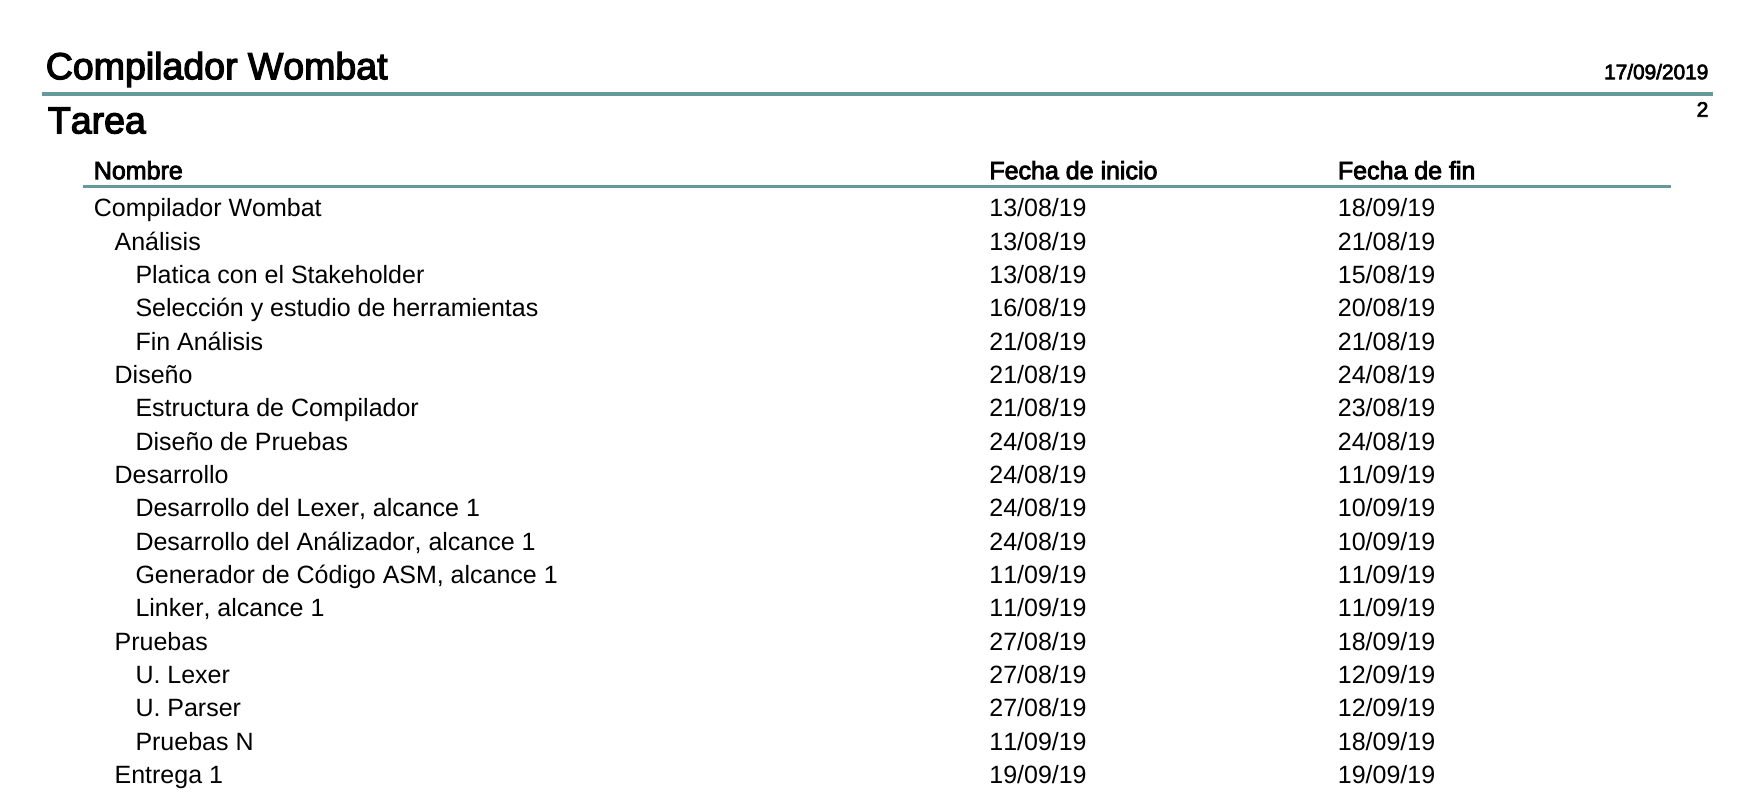
\includegraphics[width=18cm]{../img/pag-2}}
  \vspace{10mm}
  \subfigure{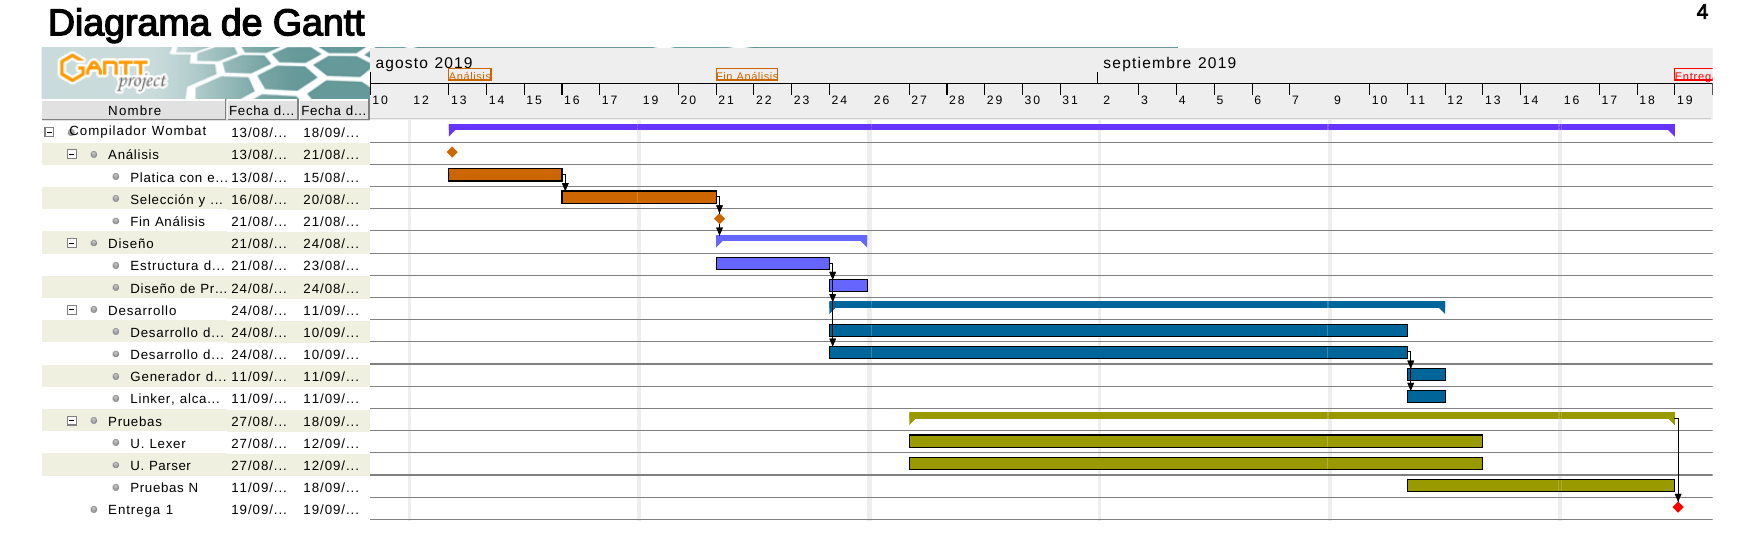
\includegraphics[width=18cm]{../img/pag-4}}
\end{figure}

\section{Arquitectura del Compilador}

La arquitectura del compilador es simple utilizado el gestor de proyectos de \textit{elixir}
\textit{mix}, la cual genera las herramientas suficientes para las pruebas y compilación. La
siguiente estructura que se decidió fue la siguiente:

\begin{itemize}
\item \_build
\item config
\item ejemplo
  \begin{itemize}
  \item return\_2.c
  \end{itemize}
\item lib
  \begin{itemize}
  \item compiladorwombat.ex
  \item wc2
    \begin{itemize}
    \item analizador.ex
    \item arbol.ex
    \item code\_gen.tex
    \item lexer.ex
    \item linker.ex
    \end{itemize}
  \item Makefile
  \item miscelanea
  \item mix.exs
  \item mix.lock
  \item README.md
  \item test
    \begin{itemize}
    \item compilador\_wombat\_test.exs
    \item stage\_1\footnote{Pruebas de Nora}
    \item test\_helper.exs
    \end{itemize}

  \end{itemize}

\end{itemize}

Ya que así se tiene separado las etapas del compilador y es fácil extender y dar mantenimiento a dicha
estructura tomando a todos los archivos necesarios de manera independiente.

\section{Plan de Pruebas y de ``Suites''}

El plan consiste en pasado un tiempo de desarrollo de los módulos del
compilador, se comenzará las pruebas mediante una  simple regla, ``Lo
que se debe de recibir, lo que se debe de mandar'', por ejemplo en el
caso del lexer, lo que este recibe es una lista de cadenas de caracteres
[``int'', ``main'', etc] y lo que debe de mandar en una lista y/o tupla de
\textit{tokens} [\textbf{:kint}, \textbf{:kmain}, etc]. Ya completado esta ``etapa''
de pruebas, se comenzará con las pruebas de \textbf{Nora}, la cual se espera solo
tener errores en sentencias especificas conservando el funcionamiento original.

\section{Conclusiones}


\end{document}
